\documentclass[11pt, spanish]{article}
\usepackage[spanish]{babel}
\selectlanguage{spanish}
\usepackage[utf8]{inputenc}
\usepackage{amsmath}
\usepackage{amsfonts}
\usepackage{amsthm}
\usepackage{float}
\usepackage{graphicx}
\pdfminorversion=5 
\pdfcompresslevel=9
\pdfobjcompresslevel=2

% Margenes
\usepackage[left=2cm,right=2cm,top=2cm,bottom=2cm]{geometry}
%Espaciado
%\linespread{1.3}


\title{Introducción al Procesamiento Digital de Imágenes - Práctica 4 (bis)}
\date{}
\author{Gonzalo Ciruelos Rodríguez (LU: 63/14)}

\begin{document}
\maketitle

Para preparar el entorno para poder ejecutar todos los programas,
primero debe tenerse instalado \texttt{python3} (y su \texttt{pip} correspondiente).
Luego, debe ejecutarse 
\begin{verbatim}
    virtualenv -p python3 venv 
    . venv/bin/activate
    pip install -r requirements.txt 
\end{verbatim}

\noindent para instalar las dependencias (pillow (para imágenes), numpy y matplotlib).



\section{Ejercicio 1.}

Transformadas de Fourier graficadas.

Modo de uso
\begin{verbatim}
    python3 practica4/ej1.py
\end{verbatim}
\end{document}

\subsection{Transformada de Fourier de dimensión 8 en 1D}

\[
\begin{bmatrix}
e^{\frac{-2 \pi i \cdot 0 \cdot 0}{8}} & e^{\frac{-2 \pi i \cdot 0 \cdot 1}{8}} & e^{\frac{-2 \pi i \cdot0 \cdot 2}{8}}
& e^{\frac{-2 \pi i \cdot 0 \cdot 3}{8}} & e^{\frac{-2 \pi i \cdot 0 \cdot 4}{8}} & e^{\frac{-2 \pi i \cdot 0 \cdot
5}{8}} & e^{\frac{-2 \pi i \cdot 0 \cdot 6}{8}} & e^{\frac{-2 \pi i \cdot 0 \cdot 7}{8}} \\
e^{\frac{-2 \pi i \cdot 1 \cdot 0}{8}} & e^{\frac{-2 \pi i \cdot 1 \cdot 1}{8}} & e^{\frac{-2 \pi i \cdot1 \cdot 2}{8}}
& e^{\frac{-2 \pi i \cdot 1 \cdot 3}{8}} & e^{\frac{-2 \pi i \cdot 1 \cdot 4}{8}} & e^{\frac{-2 \pi i \cdot 1 \cdot
5}{8}} & e^{\frac{-2 \pi i \cdot 1 \cdot 6}{8}} & e^{\frac{-2 \pi i \cdot 1 \cdot 7}{8}} \\
e^{\frac{-2 \pi i \cdot 2 \cdot 0}{8}} & e^{\frac{-2 \pi i \cdot 2 \cdot 1}{8}} & e^{\frac{-2 \pi i \cdot2 \cdot 2}{8}}
& e^{\frac{-2 \pi i \cdot 2 \cdot 3}{8}} & e^{\frac{-2 \pi i \cdot 2 \cdot 4}{8}} & e^{\frac{-2 \pi i \cdot 2 \cdot
5}{8}} & e^{\frac{-2 \pi i \cdot 2 \cdot 6}{8}} & e^{\frac{-2 \pi i \cdot 2 \cdot 7}{8}} \\
e^{\frac{-2 \pi i \cdot 3 \cdot 0}{8}} & e^{\frac{-2 \pi i \cdot 3 \cdot 1}{8}} & e^{\frac{-2 \pi i \cdot3 \cdot 2}{8}}
& e^{\frac{-2 \pi i \cdot 3 \cdot 3}{8}} & e^{\frac{-2 \pi i \cdot 3 \cdot 4}{8}} & e^{\frac{-2 \pi i \cdot 3 \cdot
5}{8}} & e^{\frac{-2 \pi i \cdot 3 \cdot 6}{8}} & e^{\frac{-2 \pi i \cdot 3 \cdot 7}{8}} \\
e^{\frac{-2 \pi i \cdot 4 \cdot 0}{8}} & e^{\frac{-2 \pi i \cdot 4 \cdot 1}{8}} & e^{\frac{-2 \pi i \cdot4 \cdot 2}{8}}
& e^{\frac{-2 \pi i \cdot 4 \cdot 3}{8}} & e^{\frac{-2 \pi i \cdot 4 \cdot 4}{8}} & e^{\frac{-2 \pi i \cdot 4 \cdot
5}{8}} & e^{\frac{-2 \pi i \cdot 4 \cdot 6}{8}} & e^{\frac{-2 \pi i \cdot 4 \cdot 7}{8}} \\
e^{\frac{-2 \pi i \cdot 5 \cdot 0}{8}} & e^{\frac{-2 \pi i \cdot 5 \cdot 1}{8}} & e^{\frac{-2 \pi i \cdot5 \cdot 2}{8}}
& e^{\frac{-2 \pi i \cdot 5 \cdot 3}{8}} & e^{\frac{-2 \pi i \cdot 5 \cdot 4}{8}} & e^{\frac{-2 \pi i \cdot 5 \cdot
5}{8}} & e^{\frac{-2 \pi i \cdot 5 \cdot 6}{8}} & e^{\frac{-2 \pi i \cdot 5 \cdot 7}{8}} \\
e^{\frac{-2 \pi i \cdot 6 \cdot 0}{8}} & e^{\frac{-2 \pi i \cdot 6 \cdot 1}{8}} & e^{\frac{-2 \pi i \cdot6 \cdot 2}{8}}
& e^{\frac{-2 \pi i \cdot 6 \cdot 3}{8}} & e^{\frac{-2 \pi i \cdot 6 \cdot 4}{8}} & e^{\frac{-2 \pi i \cdot 6 \cdot
5}{8}} & e^{\frac{-2 \pi i \cdot 6 \cdot 6}{8}} & e^{\frac{-2 \pi i \cdot 6 \cdot 7}{8}} \\
e^{\frac{-2 \pi i \cdot 7 \cdot 0}{8}} & e^{\frac{-2 \pi i \cdot 7 \cdot 1}{8}} & e^{\frac{-2 \pi i \cdot7 \cdot 2}{8}}
& e^{\frac{-2 \pi i \cdot 7 \cdot 3}{8}} & e^{\frac{-2 \pi i \cdot 7 \cdot 4}{8}} & e^{\frac{-2 \pi i \cdot 7 \cdot
5}{8}} & e^{\frac{-2 \pi i \cdot 7 \cdot 6}{8}} & e^{\frac{-2 \pi i \cdot 7 \cdot 7}{8}} \\
\end{bmatrix}
 
=

\begin{bmatrix}
e^{\frac{-0}{1} \pi i} & e^{\frac{-0}{1} \pi i} & e^{\frac{-0}{1} \pi i} & e^{\frac{-0}{1} \pi i} & e^{\frac{-0}{1} \pi
i} & e^{\frac{-0}{1} \pi i} & e^{\frac{-0}{1} \pi i} & e^{\frac{-0}{1} \pi i} \\
e^{\frac{-0}{1} \pi i} & e^{\frac{-1}{8} \pi i} & e^{\frac{-1}{4} \pi i} & e^{\frac{-3}{8} \pi i} & e^{\frac{-1}{2} \pi
i} & e^{\frac{-5}{8} \pi i} & e^{\frac{-3}{4} \pi i} & e^{\frac{-7}{8} \pi i} \\
e^{\frac{-0}{1} \pi i} & e^{\frac{-1}{4} \pi i} & e^{\frac{-1}{2} \pi i} & e^{\frac{-3}{4} \pi i} & e^{\frac{-1}{1} \pi
i} & e^{\frac{-5}{4} \pi i} & e^{\frac{-3}{2} \pi i} & e^{\frac{-7}{4} \pi i} \\
e^{\frac{-0}{1} \pi i} & e^{\frac{-3}{8} \pi i} & e^{\frac{-3}{4} \pi i} & e^{\frac{-9}{8} \pi i} & e^{\frac{-3}{2} \pi
i} & e^{\frac{-15}{8} \pi i} & e^{\frac{-9}{4} \pi i} & e^{\frac{-21}{8} \pi i} \\
e^{\frac{-0}{1} \pi i} & e^{\frac{-1}{2} \pi i} & e^{\frac{-1}{1} \pi i} & e^{\frac{-3}{2} \pi i} & e^{\frac{-2}{1} \pi
i} & e^{\frac{-5}{2} \pi i} & e^{\frac{-3}{1} \pi i} & e^{\frac{-7}{2} \pi i} \\
e^{\frac{-0}{1} \pi i} & e^{\frac{-5}{8} \pi i} & e^{\frac{-5}{4} \pi i} & e^{\frac{-15}{8} \pi i} & e^{\frac{-5}{2} \pi
i} & e^{\frac{-25}{8} \pi i} & e^{\frac{-15}{4} \pi i} & e^{\frac{-35}{8} \pi i} \\
e^{\frac{-0}{1} \pi i} & e^{\frac{-3}{4} \pi i} & e^{\frac{-3}{2} \pi i} & e^{\frac{-9}{4} \pi i} & e^{\frac{-3}{1} \pi
i} & e^{\frac{-15}{4} \pi i} & e^{\frac{-9}{2} \pi i} & e^{\frac{-21}{4} \pi i} \\
e^{\frac{-0}{1} \pi i} & e^{\frac{-7}{8} \pi i} & e^{\frac{-7}{4} \pi i} & e^{\frac{-21}{8} \pi i} & e^{\frac{-7}{2} \pi
i} & e^{\frac{-35}{8} \pi i} & e^{\frac{-21}{4} \pi i} & e^{\frac{-49}{8} \pi i} \\
\end{bmatrix}
\]

\begin{figure}[H]
\centering
  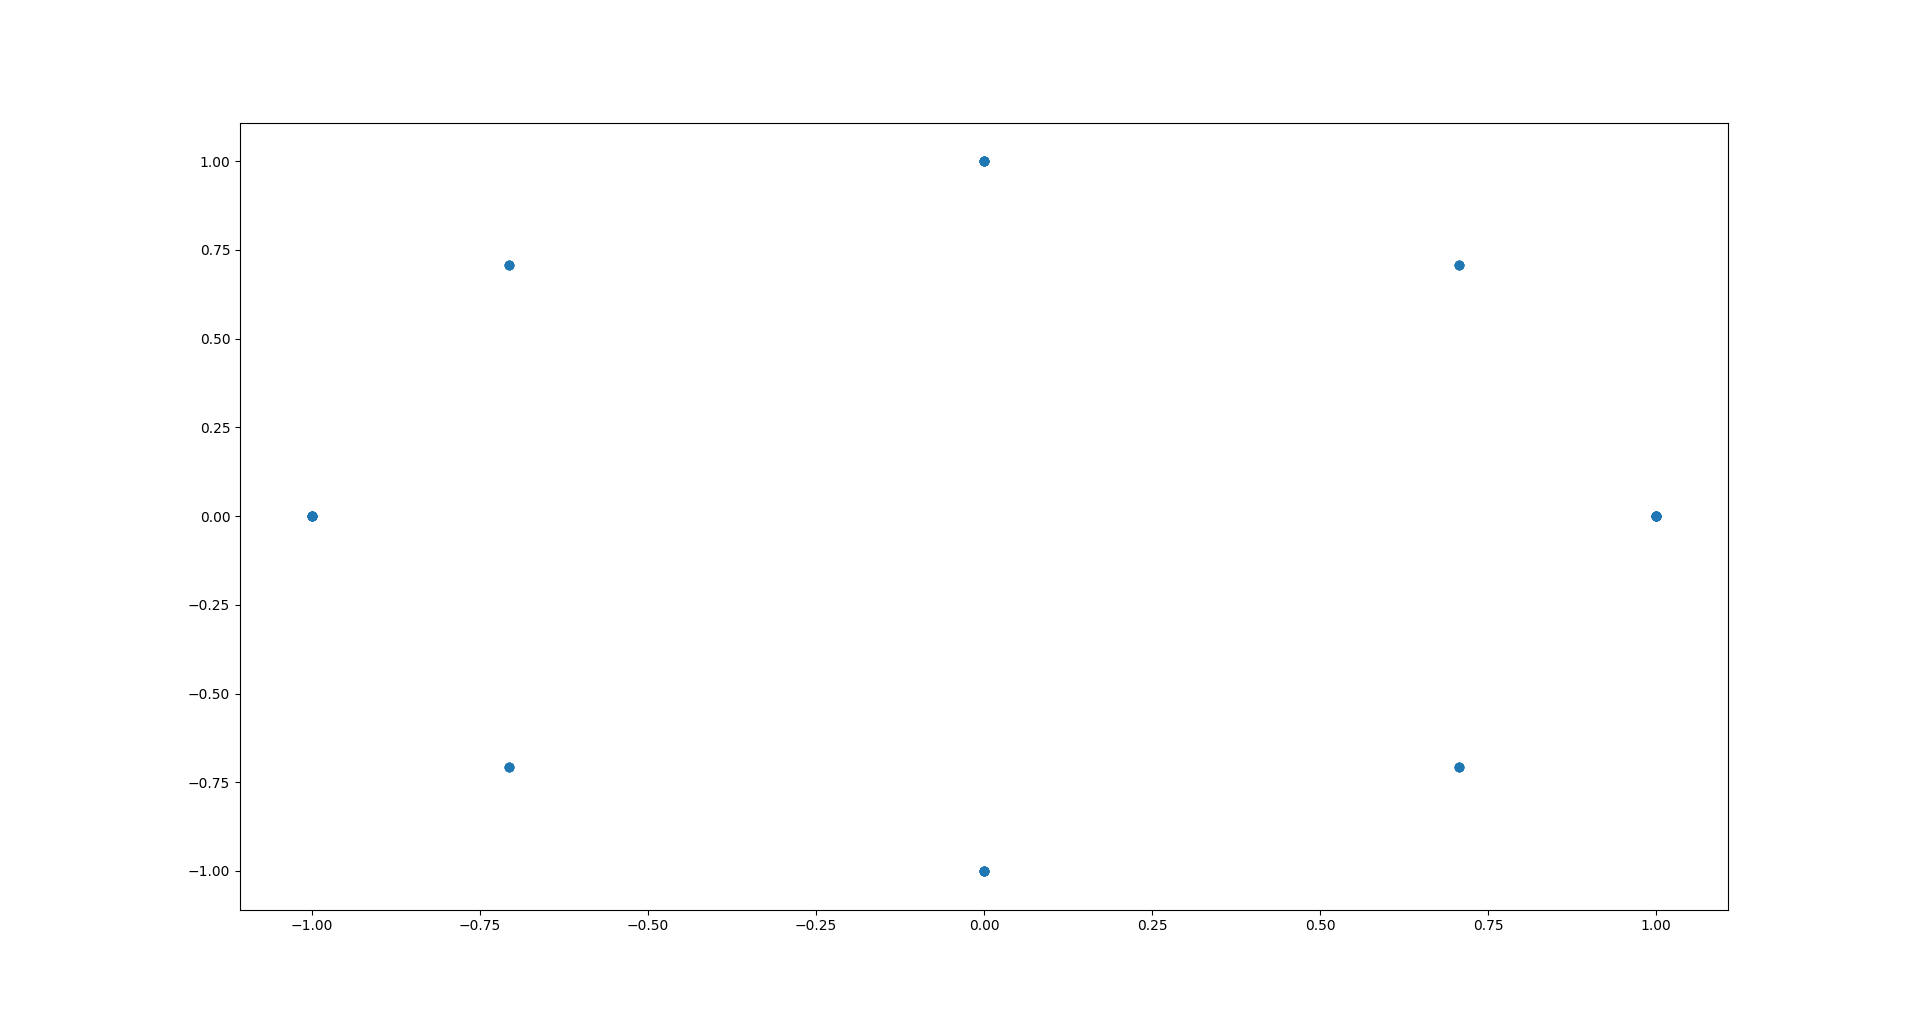
\includegraphics[height=6cm]{informe-imgs/ej1.png}
  \caption{\texttt{python3 practica4/ej1.py}}
\end{figure}

